\documentclass[a4paper]{beamer}
\usepackage{beamerthemePadovaDEI}

\usepackage[utf8]{inputenc}
\usepackage[T1]{fontenc}
\usepackage{mathtools}
\usepackage{lmodern}
\usepackage{textcomp}
\usepackage{subcaption}
\captionsetup{compatibility=false}
\usepackage[italian]{babel}

\title[title]{Esperimenti MIP per una classe di\\problemi di assegnamento quadratico}
\author[Persone]{Laureando: Mattia Toffolon\\Relatore: Prof. Domenico Salvagnin}
\date{\small \textit{Padova, 18 luglio 2023}}

\begin{document}
%
%% title
\begin{frame}
\maketitle
\end{frame}

\begin{frame}{Indice}
	\begin{itemize}
		\item Introduzione al problema di assegnamento quadratico
		\vfill
		\item Istanze Tai*c
		\vfill
		\item Modellazione algebrica
		\vfill
		\item Risultati sperimentali
		\vfill
		\item Conclusioni
		\vfill
	\end{itemize}
\end{frame}

\begin{frame}{Quadratic assignment problem}
Il problema di ottimizzazione di assegnamento quadratico (QAP) consiste nell'assegnare \textbf{\textit{n} unità} in 
\textbf{\textit{n} posizioni} differenti. 

Sono noti il flusso di informazioni da trasferire da ogni unità alle altre
e per ogni coppia di posizioni la distanza che le separa.
\newline \newline
L'assegnamento ottimale è quello che rende \textbf{minima} la \textbf{somma dei prodotti flusso x distanza} relativi ad ogni coppia
di unità.
\newline \newline
Matematicamente, il problema può essere espresso come segue
\begin{align*}
    \min_{\pi \, \in \, P(n)} \sum_{i\,=\,1}^{n} \sum_{j=1}^{n} a_{ij} b_{\pi_{i} \pi_{j}}
\end{align*}
\end{frame}

\begin{frame}{Istanze Tai*c}
La classe di problemi QAP studiata è quella delle istanze Tai*c.
\newline \newline
Queste posso essere generate tramite il metodo "Densità di grigio".
Esso si fonda sull'utilizzo di una griglia $n_1\times n_2 \,(=n)$ dalla quale è possibile ricavare i parametri di distanza.
Quelli di flusso invece, sono a valore unitario o nullo in base alla densità considerata.
\begin{figure}[h!]
    \centering
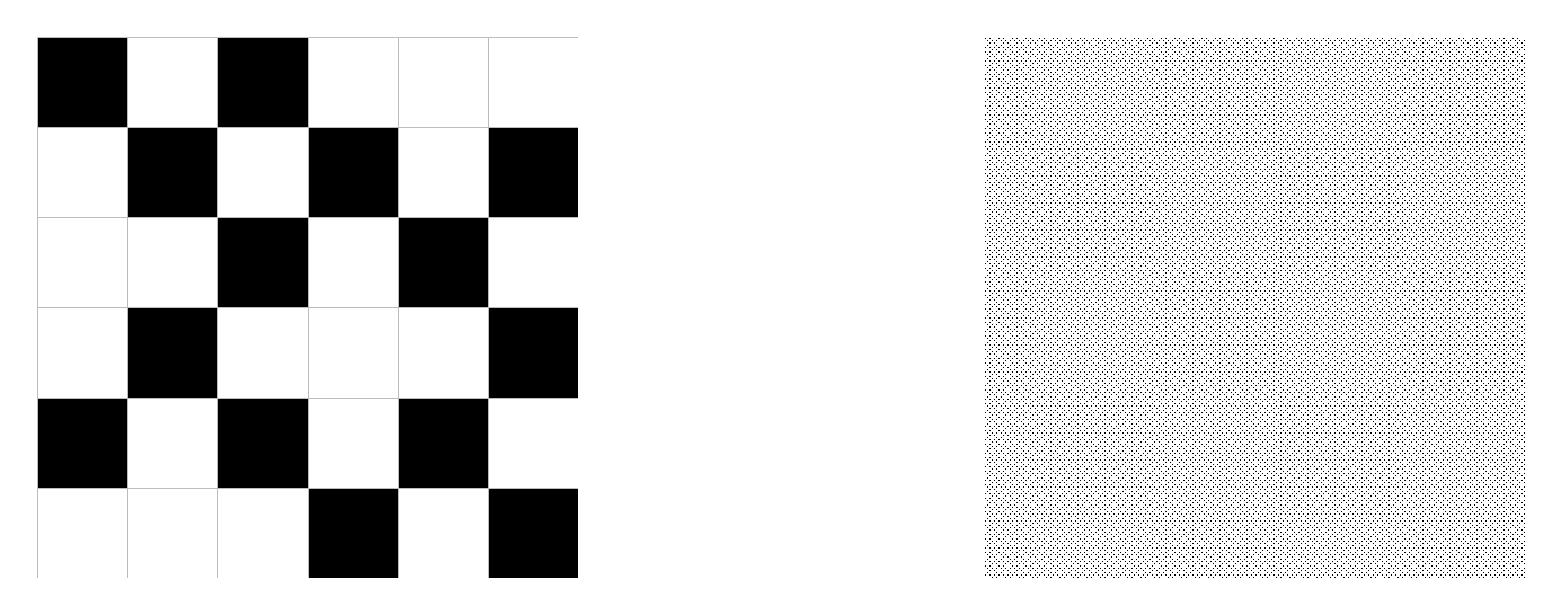
\includegraphics[scale=0.12]{images/gray_36_40.png}
\caption{Esempio di griglia "Densità di grigio" ed un suo possibile utilizzo}
\end{figure}    
\end{frame}

\begin{frame}{Modellazione algebrica}
Le diverse fasi in cui si è articolata la modellazione algebrica del problema di ottimizzazione sono state:
\begin{itemize}
\item individuazione degli insiemi
\item individuazione dei parametri
\item individuazione delle variabili
\item definizione dei vincoli e della funzione obiettivo
\item linearizzazione del modello 
\item semplificazione del modello
\end{itemize}
\vfill
Le ultime due fasi sono state necessarie per portare il modello in forma MIP e per ridurre il costo computazionale richiesto 
per risolvere le istanze.
\end{frame}

\begin{frame}{Modellazione algebrica}
Il modello risultante dalla modellazione algebrica è il seguente:
\begin{align*}
	\begin{array}{l}
      \min \, \sum_{i\in I} \sum_{j\in I} \, b_{ij}\cdot y_{ij} \\
      \sum_{i\in I} \, x_{i} = n_1 \\
      y_{ij} \, \leq \, x_{i}   \;\;\;\qquad \forall \; i,j \in I \\ 
      y_{ij} \, \leq \, x_{j}   \;\;\;\qquad \forall \; i,j \in I \\
      y_{ij} \, \geq \, x_{i} + x_{j} - 1      \,\qquad \forall \; i,j \in I\\
      x_{i} ,\, y_{ij} \in \{0,1\}      \;\quad\qquad \forall \; i,j \in I
    \end{array}
\end{align*}
\vfill
Si nota come, dato \textit{n} il numero di unità e di posizioni, è necessario prendere in esame $n^2$ variabili. 
Deriva da qui l'elevata complessità di risoluzione delle istanze del problema.

\end{frame}

\begin{frame}{Ringraziamenti}
\centering
\LARGE Grazie per l'attenzione!
\end{frame}

\begin{frame}
\maketitle
\end{frame}

\end{document}